% !TeX root = ../main.tex

\chapter{Device design and dispersion engineering of nonlinear ring cavities}

Mentioned above, %before the design of ring resonators, 
second-order mode dispersion $ D_2 $ is the key factor in phase matching condition, especially in frequency mismatch. In this case, a typical approach to reduce the dispersion offset is balancing the intrinsic material dispersion and structure induced dispersion---waveguide dispersion. This method is usually named as dispersion compensation. Typically, it requires greater film thickness which complicates the fabrication process, such as thicker film deposition and high-selectivity etching. Besides, it only suitable for simple rectangular channel waveguides.

Furthermore, in some structures including slot waveguides, the waveguide dispersion features flat curvature in a appropriate dimension, indicating that by optimizing the structure, the material dispersion can be not only compensated but also flattened. Another example is mode crossing, the avoiding crossing of dispersion curve, leads to local dispersion inversion even in a thin thickness. 

In this chapter, above methods are described sequentially for the specific silicon nitride ring resonators. Beside, in the case of ring resonators, to improve the coupling efficiency, design of mode size convertors at bus waveguide input/output ports is also introduced.

\section{Dispersion compensation}\label{sec:disp-comp}
indicated in \autoref{eq:te-eq}, the dispersion behavior of integrated devices is not only the intrinsic material property, but also depends on the waveguide dimension. Thus, the phase mismatch origins as a result of both material dispersion $D_M$ and waveguide dispersion $ D_W $, $D_{\lambda}= D_M + D_W$. Here, we adopt the wavelength dispersion parameter since the wavelength domain is measurable.

Usually, the Sellmeier equation is used to fit the refractive index for a particular transparent medium based on the Lorentz-Drude mode. \citeauthor{Luke2015a} reported the below measured refractive index of stoichiomertric \ce{Si3N4} film \cite{Luke2015a}
\begin{equation}\label{eq:si3n4-selleimeier}
    n_{\ce{Si3N4}}^2 = 1 + \frac{3.0249 \lambda^2}{\lambda^2-135.3406^2} + \frac{40314 \lambda^2}{\lambda^2 - 1239842^2}
\end{equation}

This Sellmeier equation is valid over the wavelength range 310–5504 \si{\nm}.
The result of \autoref{eq:si3n4-selleimeier} is plotted in \autoref{fig:Luke-si3n4}, along with the material dispersion parameter $D_M$, which is calculated at the precision of \si{\nm} using the second-order finite difference of refractive index. In the telecom C-band 1550 nm, $n$=1.9963 and $D_M$ = -6.57 \dispu, which suggests the material dispersion at this range is considerably small. To note, the Sellmeier equation used above is valid only for dehydrogenated shoichiomertric silicon nitride. In most cases of common film growing, deposition sources and methods influence the refractive index significantly.

\begin{figure}
    \centering
    \includesvg{luke/Luke}
    \mycaption{Refractive index and dispersion parameter measured in reference}{$ \lambda$=1550 \si{\nm}, $n$=1.9963 and $D_M$ = -6.5656 \dispu .}
    \label{fig:Luke-si3n4}
\end{figure}
To evaluate the waveguide dispersion parameter, the numerical simulation using commercial software \si{\nm}{Lumerical MODE} is adopted to solve the modes and sweep the cross section dimension in a channel waveguide. The selected mode is fundamental TE modes, and the bent radius 200 \um is involved in the mode solver.

Shown in \autoref{fig:wg-disp}, the dimension dependence of waveguide dispersion features negative values in a small size, i.e. behaving normal dispersion at the second order. Nevertheless, as either the thickness or width increases,
$D_W$ turns positive. This indicates that to achieve zero dispersion in phase match condition of four wave mixing, the normal material dispersion can be compensated with anomalous waveguide dispersion. 
For example, at 1550 \si{\nm}, in a 1.5-\si{\um}-wide and 0.8-\si{\um}-thick silicon nitride waveguide cladded by silica, where the refractive index is 1.48,
the waveguide dispersion is 122.56 \dispu. Substituting into the second-order dispersion chain rule in \autoref{eq:disp-chain}, the second-order mode number dispersion parameter $ D_2 $ is about 3.07 MHz.

%It is close to zero dispersion for the pump wavelength.

\begin{figure}
	\centering
	\includesvg{wg_disp/fdtd_fine}
	\mycaption{Waveguide dispersion map simulated by Lumerical MODE}{The central wavelength to perform the simulation is 1550 \si{\nm} and the precision is nm. We select the fundamental TE mode as the objective to study the waveguide dispersion. The scattered point in the figure is 1.5-\si{\um}-wide and 0.8-\si{\um}-thick.}
	\label{fig:wg-disp}
\end{figure}

\section[{Dispersion engineering using slot structure}]{Dispersion engineering using \\ slot structure}

The slot waveguide was firstly realized by \citeauthor{Xu2004} experimentally \cite{Xu2004}. The same group, \citeauthor{Almeida2004} then discussed the light enhancement and confinement caused by large discontinuity of the electric field at high-index-contrast interfaces \cite{Almeida2004}. In the recent decade, it is fully studied that such a novel waveguide can be also used to design dispersion-flattened waveguide \cites{Mas2010, Zhang2010, Zhu2012, Nolte2013}, including the both vertical or horizontal and single or multiple slots. It is also reported a micro-ring resonators formed by a slot hybrid waveguide 
exhibits a flat and low anomalous dispersion \cite{Zhang2013}.

In our research, the vertical slot is preferred due to the easy fabrication during the monolithic process. 
%We propose a double-slot silicon nitride to achieve near-zero and flat dispersion.
For example, in a double vertical slot waveguide illustrated in \autoref{fig:slot-illus}, two extra gaps are fully etched and then reburied with low-index medium instead. 
Except the waveguide width $w$ and thickness $t$, two extra parameters are defined, the position factor $ \mathit{pf} $, ratio of slot position to the waveguide width $w$, and the filling factor $ \mathit{ff} $, ratio of slot width to the waveguide width.

\begin{figure}
		\centering	
		\includesvg[width=3in]{slot/slot_illus}
		\mycaption{Illustration of a double vertical slot waveguide}{The cyan region is \ce{Si3N4} waveguide and surrounded by silica.}
		\label{fig:slot-illus}
\end{figure}


\begin{figure}
	\centering
%	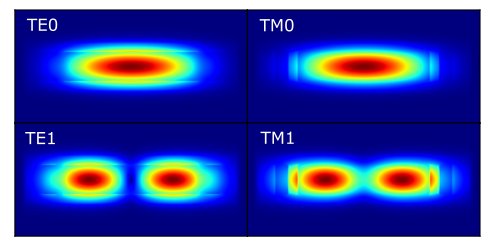
\includegraphics[width=.8\linewidth]{imgs/png/slot_mode}
	\includesvg[width=4in]{slot/slot_mode}
    \mycaption{Modes of the double vertical slot waveguide}{$w$=2.5, $t$=0.8, $\mathit{ff}$=0.053, $\mathit{pf}$=0.4}
 	\label{fig:slot-mode}
\end{figure}

%\begin{figure}
%	\centering
%	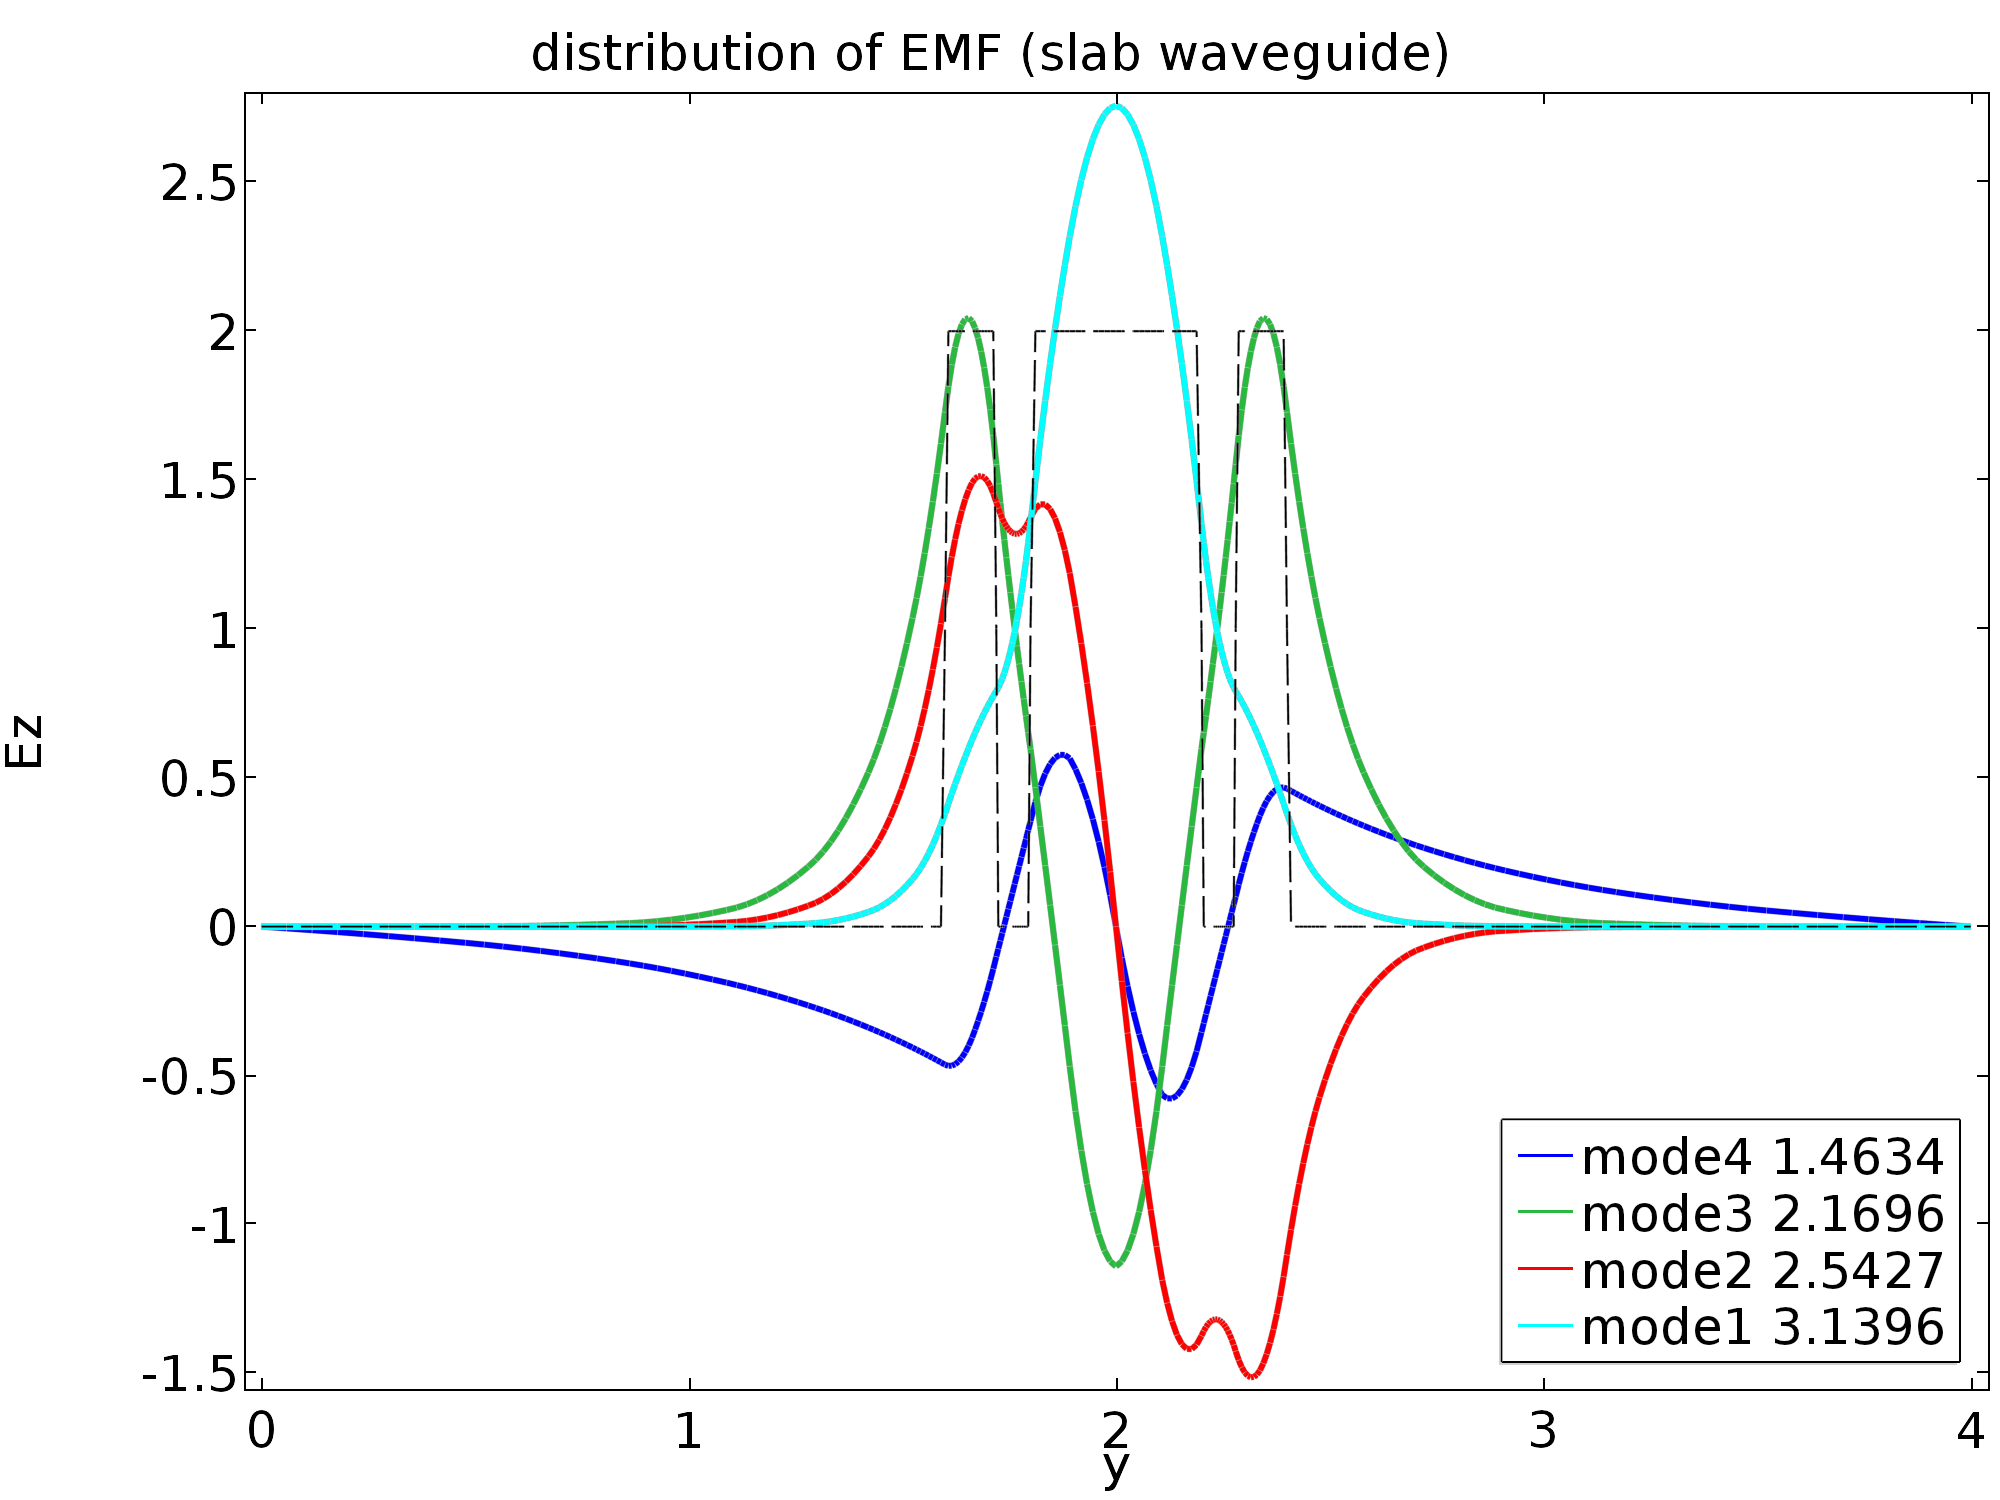
\includegraphics[width=0.7\linewidth]{imgs/png/Ez}
%	\mycaption{Modes of the double vertical slot waveguide}{}
%	\label{fig:slot-mode-Ez}
%\end{figure}

To classify the modes in this slot structure, the same mode solver mention in previous section is performed.
In the result shown in \autoref{fig:slot-mode}, in TM0 and TM1 modes, the light is confined strongly in the slots while the TE0 and TE1 is similar to the normal TE modes, where the discontinuity is obvious on the upper and lower interfaces.

%An interesting finding is that differing from the simple rectangular waveguide, 
%the mode of both quasi-TE and quasi-TM modes can be assumed as the symmetric and anti-symmetric combination of the mode field on both sides. 

%\begin{align}\label{key}
%	\vb{E}_\mathrm{sym} &= \vb{E}_{l} + \vb{E}_{r} \\
%	\vb{E}_\mathrm{asym} &= \vb{E}_{l} - \vb{E}_{r} \nonumber
%\end{align}

%\autoref{fig:slot-mode-Ez} is the \textit{z}-component of the electric field of the four modes. For example, quasi-TE0 mode is even parity while quasi-TE1 mode is odd parity.

Furthermore, by optimizing the position and filling factors, the near-zero and flattened dispersion can be obtained. 


\section{Effects of mode crossing}

In the conclusion of \autoref{sec:disp-comp},
only in the wider or thicker waveguides can the zero dispersion be compensated. However, 
despite the fabrication difficulty arising from thicker films,
the waveguide of larger size also supports high order modes. 

In this case, due to the perturbation of high order modes, the linear mode coupling occurs and influences the resonance spectrum. 
In the study of soliton generation,
it is found that avoided mode crossings induced by linear mode coupling can prevent optical soliton formation when affecting resonator modes close to the pump laser frequency \cites{Herr2014a,Bao2018}. On the other hand, by introducing artificial mode crossing, the anomalous group velocity can also be achieved \cite{Kim2017}. Even though the phenomena mentioned in these works are classical, but in the term of phase matching condition, the physics is similar.

In the following research, the mode crossings found in our devices not only change the spectrum transmission, but also leads to failure of evaluating the dispersion properties.


\section{Edge coupling}
Much of related works, such as photonic crystals or whispering gallery mode resonators, use prism coupling or tapered fiber coupling for tunability of coupling condition. 
%interact the external optical filed with cavity evanescent filed though, 
In the case of integrated ring resonators, the bus wavegudies are designed in the distance of several gaps, usually varying from under coupling to over coupling. 
Thus, the light confined in the bus waveguide can be directly coupled inwards or outwards using appropriate optical fibers. 
In previous works \cite{Sunada2018}, both grating coupling and edge coupling were adopted. However, considering the broadband frequency conversion motivation, the edge coupling is preferred for a comparatively broader 3dB bandwidth.

To achieve high coupling efficiency, inverted tapered couplers are used as mode convertor. The input and output ports of waveguide are both tapered from normal width 1.5 \um to a narrower end. By FDTD methods, the mode field is swept with different taper end widths.

\begin{figure}
	\centering
	\begin{subfigure}[b]{0.33\textwidth}
		\includesvg[width=\textwidth]{taper/03.svg}
		\caption{End width 0.3 \um}
	\end{subfigure}\hfill
	\begin{subfigure}[b]{0.33\textwidth}
		\includesvg[width=\textwidth]{taper/06}
		\caption{End width 0.6 \um}
	\end{subfigure}\hfill
	\begin{subfigure}[b]{0.33\textwidth}
		\includesvg[width=\textwidth]{taper/09}
		\caption{End width 0.9 \um}
	\end{subfigure}
	\vfill
	\begin{subfigure}[b]{0.33\textwidth}
		\includesvg[width=\textwidth]{taper/12}
		\caption{End width 1.2 \um}
	\end{subfigure}
	\begin{subfigure}[b]{0.33\textwidth}
		\includesvg[width=\textwidth]{taper/15}
		\caption{End width 1.5 \um}
	\end{subfigure}
	\mycaption{Mode field at the taper end}{The outline of taper edge is profiled.}
	\label{fig:taper}
\end{figure}

From the result shown in \autoref{fig:taper}a, the mode fields expand horizontally as the taper end width increases proportionally. The largest mode size of 3.4 \um $\times$ 3.4 \um is successfully demonstrated, but the enhancement is not significant compared with no tapered port in \autoref{fig:taper}e. In result, a lensed fiber with spot diameter from 3.0 \um  to 3.4 \um  is recommended. 



